%%
% Copyright (c) 2017 - 2020, Pascal Wagler;
% Copyright (c) 2014 - 2020, John MacFarlane
%
% All rights reserved.
%
% Redistribution and use in source and binary forms, with or without
% modification, are permitted provided that the following conditions
% are met:
%
% - Redistributions of source code must retain the above copyright
% notice, this list of conditions and the following disclaimer.
%
% - Redistributions in binary form must reproduce the above copyright
% notice, this list of conditions and the following disclaimer in the
% documentation and/or other materials provided with the distribution.
%
% - Neither the name of John MacFarlane nor the names of other
% contributors may be used to endorse or promote products derived
% from this software without specific prior written permission.
%
% THIS SOFTWARE IS PROVIDED BY THE COPYRIGHT HOLDERS AND CONTRIBUTORS
% "AS IS" AND ANY EXPRESS OR IMPLIED WARRANTIES, INCLUDING, BUT NOT
% LIMITED TO, THE IMPLIED WARRANTIES OF MERCHANTABILITY AND FITNESS
% FOR A PARTICULAR PURPOSE ARE DISCLAIMED. IN NO EVENT SHALL THE
% COPYRIGHT OWNER OR CONTRIBUTORS BE LIABLE FOR ANY DIRECT, INDIRECT,
% INCIDENTAL, SPECIAL, EXEMPLARY, OR CONSEQUENTIAL DAMAGES (INCLUDING,
% BUT NOT LIMITED TO, PROCUREMENT OF SUBSTITUTE GOODS OR SERVICES;
% LOSS OF USE, DATA, OR PROFITS; OR BUSINESS INTERRUPTION) HOWEVER
% CAUSED AND ON ANY THEORY OF LIABILITY, WHETHER IN CONTRACT, STRICT
% LIABILITY, OR TORT (INCLUDING NEGLIGENCE OR OTHERWISE) ARISING IN
% ANY WAY OUT OF THE USE OF THIS SOFTWARE, EVEN IF ADVISED OF THE
% POSSIBILITY OF SUCH DAMAGE.
%%

%%
% This is the Eisvogel pandoc LaTeX template.
%
% For usage information and examples visit the official GitHub page:
% https://github.com/Wandmalfarbe/pandoc-latex-template
%%

\DeclareUnicodeCharacter{2212}{-}

% Options for packages loaded elsewhere
\PassOptionsToPackage{unicode}{hyperref}
\PassOptionsToPackage{hyphens}{url}
\PassOptionsToPackage{dvipsnames,svgnames*,x11names*,table}{xcolor}
%
\documentclass[
  12pt,
  a4paper,
,tablecaptionabove
]{scrartcl}
\usepackage{lmodern}
\usepackage{setspace}
\setstretch{1.2}
\usepackage{amssymb,amsmath}
\usepackage{ifxetex,ifluatex}
\ifnum 0\ifxetex 1\fi\ifluatex 1\fi=0 % if pdftex
  \usepackage[T1]{fontenc}
  \usepackage[utf8]{inputenc}
  \usepackage{textcomp} % provide euro and other symbols
\else % if luatex or xetex
  \usepackage{unicode-math}
  \defaultfontfeatures{Scale=MatchLowercase}
  \defaultfontfeatures[\rmfamily]{Ligatures=TeX,Scale=1}
\fi
% Use upquote if available, for straight quotes in verbatim environments
\IfFileExists{upquote.sty}{\usepackage{upquote}}{}
\IfFileExists{microtype.sty}{% use microtype if available
  \usepackage[]{microtype}
  \UseMicrotypeSet[protrusion]{basicmath} % disable protrusion for tt fonts
}{}
\makeatletter
\@ifundefined{KOMAClassName}{% if non-KOMA class
  \IfFileExists{parskip.sty}{%
    \usepackage{parskip}
  }{% else
    \setlength{\parindent}{0pt}
    \setlength{\parskip}{6pt plus 2pt minus 1pt}}
}{% if KOMA class
  \KOMAoptions{parskip=half}}
\makeatother
\usepackage{xcolor}
\definecolor{default-linkcolor}{HTML}{A50000}
\definecolor{default-filecolor}{HTML}{A50000}
\definecolor{default-citecolor}{HTML}{4077C0}
\definecolor{default-urlcolor}{HTML}{4077C0}
\IfFileExists{xurl.sty}{\usepackage{xurl}}{} % add URL line breaks if available
\IfFileExists{bookmark.sty}{\usepackage{bookmark}}{\usepackage{hyperref}}
\hypersetup{
  hidelinks,
  breaklinks=true,
  pdfcreator={LaTeX via pandoc with the Eisvogel template}}
\urlstyle{same} % disable monospaced font for URLs
\usepackage[margin=1in]{geometry}
\usepackage{longtable,booktabs}
% Correct order of tables after \paragraph or \subparagraph
\usepackage{etoolbox}
\makeatletter
\patchcmd\longtable{\par}{\if@noskipsec\mbox{}\fi\par}{}{}
\makeatother
% Allow footnotes in longtable head/foot
\IfFileExists{footnotehyper.sty}{\usepackage{footnotehyper}}{\usepackage{footnote}}
\makesavenoteenv{longtable}
% add backlinks to footnote references, cf. https://tex.stackexchange.com/questions/302266/make-footnote-clickable-both-ways
\usepackage{footnotebackref}
\usepackage{graphicx}
\makeatletter
\def\maxwidth{\ifdim\Gin@nat@width>\linewidth\linewidth\else\Gin@nat@width\fi}
\def\maxheight{\ifdim\Gin@nat@height>\textheight\textheight\else\Gin@nat@height\fi}
\makeatother
% Scale images if necessary, so that they will not overflow the page
% margins by default, and it is still possible to overwrite the defaults
% using explicit options in \includegraphics[width, height, ...]{}
\setkeys{Gin}{width=\maxwidth,height=\maxheight,keepaspectratio}
\setlength{\emergencystretch}{3em}  % prevent overfull lines
\providecommand{\tightlist}{%
  \setlength{\itemsep}{0pt}\setlength{\parskip}{0pt}}
\setcounter{secnumdepth}{-\maxdimen} % remove section numbering

% Make use of float-package and set default placement for figures to H.
% The option H means 'PUT IT HERE' (as  opposed to the standard h option which means 'You may put it here if you like').
\usepackage{float}
\floatplacement{figure}{H}

\usepackage{booktabs}
\usepackage{longtable}
\usepackage{array}
\usepackage{multirow}
\usepackage{wrapfig}
\usepackage{float}
\usepackage{colortbl}
\usepackage{pdflscape}
\usepackage{tabu}
\usepackage{threeparttable}
\usepackage{threeparttablex}
\usepackage[normalem]{ulem}
\usepackage{makecell}
\usepackage{xcolor}
\usepackage{lineno}
\linenumbers

\newlength{\cslhangindent}
\setlength{\cslhangindent}{1.5em}
\newlength{\csllabelwidth}
\setlength{\csllabelwidth}{3em}
\newenvironment{CSLReferences}[2] % #1 hanging-ident, #2 entry spacing
 {% don't indent paragraphs
  \setlength{\parindent}{0pt}
  % turn on hanging indent if param 1 is 1
  \ifodd #1 \everypar{\setlength{\hangindent}{\cslhangindent}}\ignorespaces\fi
  % set entry spacing
  \ifnum #2 > 0
  \setlength{\parskip}{#2\baselineskip}
  \fi
 }%
 {}
\usepackage{calc}
\newcommand{\CSLBlock}[1]{#1\hfill\break}
\newcommand{\CSLLeftMargin}[1]{\parbox[t]{\csllabelwidth}{#1}}
\newcommand{\CSLRightInline}[1]{\parbox[t]{\linewidth - \csllabelwidth}{#1}\break}
\newcommand{\CSLIndent}[1]{\hspace{\cslhangindent}#1}

\date{}


%%
%% added
%%

%
% language specification
%
% If no language is specified, use English as the default main document language.
%

\ifnum 0\ifxetex 1\fi\ifluatex 1\fi=0 % if pdftex
  \usepackage[shorthands=off,main=english]{babel}
\else
    % Workaround for bug in Polyglossia that breaks `\familydefault` when `\setmainlanguage` is used.
  % See https://github.com/Wandmalfarbe/pandoc-latex-template/issues/8
  % See https://github.com/reutenauer/polyglossia/issues/186
  % See https://github.com/reutenauer/polyglossia/issues/127
  \renewcommand*\familydefault{\sfdefault}
    % load polyglossia as late as possible as it *could* call bidi if RTL lang (e.g. Hebrew or Arabic)
  \usepackage{polyglossia}
  \setmainlanguage[]{english}
\fi



%
% for the background color of the title page
%

%
% break urls
%
\PassOptionsToPackage{hyphens}{url}

%
% When using babel or polyglossia with biblatex, loading csquotes is recommended
% to ensure that quoted texts are typeset according to the rules of your main language.
%
\usepackage{csquotes}

%
% captions
%
%\definecolor{caption-color}{HTML}{777777}
\definecolor{caption-color}{HTML}{37474F}
%\usepackage[font={stretch=1.2}, textfont={color=caption-color}, position=top, skip=4mm, labelfont=bf, singlelinecheck=false, justification=raggedright]{caption}
\usepackage[font={stretch=1}, textfont={color=caption-color}, position=top, skip=2mm, labelfont=bf, singlelinecheck=false, justification=raggedright]{caption}
\setcapindent{0em}

%
% blockquote
%
\definecolor{blockquote-border}{RGB}{221,221,221}
\definecolor{blockquote-text}{RGB}{119,119,119}
\usepackage{mdframed}
\newmdenv[rightline=false,bottomline=false,topline=false,linewidth=3pt,linecolor=blockquote-border,skipabove=\parskip]{customblockquote}
\renewenvironment{quote}{\begin{customblockquote}\list{}{\rightmargin=0em\leftmargin=0em}%
\item\relax\color{blockquote-text}\ignorespaces}{\unskip\unskip\endlist\end{customblockquote}}

%
% Source Sans Pro as the de­fault font fam­ily
% Source Code Pro for monospace text
%
% 'default' option sets the default
% font family to Source Sans Pro, not \sfdefault.
%
\ifnum 0\ifxetex 1\fi\ifluatex 1\fi=0 % if pdftex
    \usepackage[default]{sourcesanspro}
  \usepackage{sourcecodepro}
  %\usepackage{}
  \else % if not pdftex
    \usepackage[default]{sourcesanspro}
  \usepackage{sourcecodepro}
  %\usepackage{}

  % XeLaTeX specific adjustments for straight quotes: https://tex.stackexchange.com/a/354887
  % This issue is already fixed (see https://github.com/silkeh/latex-sourcecodepro/pull/5) but the
  % fix is still unreleased.
  % TODO: Remove this workaround when the new version of sourcecodepro is released on CTAN.
  \ifxetex
    \makeatletter
    \defaultfontfeatures[\ttfamily]
      { Numbers   = \sourcecodepro@figurestyle,
        Scale     = \SourceCodePro@scale,
        Extension = .otf }
    \setmonofont
      [ UprightFont    = *-\sourcecodepro@regstyle,
        ItalicFont     = *-\sourcecodepro@regstyle It,
        BoldFont       = *-\sourcecodepro@boldstyle,
        BoldItalicFont = *-\sourcecodepro@boldstyle It ]
      {SourceCodePro}
    \makeatother
  \fi
  \fi

%
% heading color
%
\definecolor{heading-color}{RGB}{40,40,40}
\addtokomafont{section}{\color{heading-color}}
% When using the classes report, scrreprt, book,
% scrbook or memoir, uncomment the following line.
%\addtokomafont{chapter}{\color{heading-color}}

%
% variables for title and author
%
\usepackage{titling}
\title{}
\author{}

%
% tables
%

\definecolor{table-row-color}{HTML}{F5F5F5}
\definecolor{table-rule-color}{HTML}{999999}

%\arrayrulecolor{black!40}
\arrayrulecolor{table-rule-color}     % color of \toprule, \midrule, \bottomrule
\setlength\heavyrulewidth{0.3ex}      % thickness of \toprule, \bottomrule
\renewcommand{\arraystretch}{1.3}     % spacing (padding)


%
% remove paragraph indention
%
\setlength{\parindent}{0pt}
\setlength{\parskip}{6pt plus 2pt minus 1pt}
\setlength{\emergencystretch}{3em}  % prevent overfull lines

%
%
% Listings
%
%


%
% header and footer
%
\usepackage{fancyhdr}

\fancypagestyle{eisvogel-header-footer}{
  \fancyhead{}
  \fancyfoot{}
  \lhead[]{}
  \chead[]{}
  \rhead[]{}
  %\lfoot[\thepage]{}
  \cfoot[]{}
  \cfoot[]{\thepage}
  \renewcommand{\headrulewidth}{0.0pt}
 % \renewcommand{\footrulewidth}{0.0pt}
 % \renewcommand{\headrulewidth}{0.4pt}
 % \renewcommand{\footrulewidth}{0.4pt}
}
\pagestyle{eisvogel-header-footer}

%%
%% end added
%%

\begin{document}

%%
%% begin titlepage
%%

%%
%% end titlepage
%%



Sources and consequences of mismatch between leaf disc and whole-leaf
leaf mass per area (LMA)

\[ \]

Phisamai Maenpuen\textsuperscript{1,2,3}, Masatoshi
Katabuchi\textsuperscript{1*}, Yusuke Onoda\textsuperscript{4}, Cong
Zhou\textsuperscript{1,2}, Jiao-Lin Zhang\textsuperscript{1,3*}, Ya-Jun
Chen\textsuperscript{1,3,5}

\[ \]

\textsuperscript{1} CAS Key Laboratory of Tropical Forest Ecology,
Xishuangbanna Tropical Botanical Garden, Chinese Academy of Sciences,
Menglun, Yunnan 666303, China

\textsuperscript{2} University of Chinese Academy of Sciences, Beijing
100049, China

\textsuperscript{3} Center of Plant Ecology, Core Botanical Gardens,
Chinese Academy of Sciences, Yunnan 666303, China

\textsuperscript{4} Graduate School of Agriculture, Kyoto University,
Kyoto 606-8502, Japan

\textsuperscript{5} Savanna Ecosystem Research Station, Xishuangbanna
Tropical Botanical Garden, Chinese Academy of Sciences, Yuanjiang,
Yunnan 6663300, China

\[ \]

\textbf{Corresponding Authors}:

Masatoshi Katabuchi

E-mail:
\href{mailto:mattocci27@gmail.com}{\nolinkurl{mattocci27@gmail.com}}

Jiao-Lin Zhang

Tel: +86 691 871 3046; Fax: +86 691 871 5070; E-mail:
\href{mailto:zjl@xtbg.org.cn}{\nolinkurl{zjl@xtbg.org.cn}}

\[ \]

Manuscript received \_\_\_\_\_\_\_; revision accepted \_\_\_\_\_\_\_.

\textbf{Running title}: Leaf disc and whole-leaf LMA

\newpage

\hypertarget{abstract}{%
\section{ABSTRACT}\label{abstract}}

\textbf{PREMISE:} Leaf mass per area (LMA), which is the key trait in
leaf economic spectrum and plant growth analysis, is measured from leaf
discs or whole leaves. These differences in the measurement methods may
lead to large differences in the estimates of LMA values.

\textbf{METHODS:} We determined LMA using leaf discs and whole-leaf
(including petiole) for 334 woody species from a wide range of biomes
(tropics, subtropics, savanna, and temperate) to examine what extent
whole-leaf and leaf disc LMA match, whether the differences in the
estimates are associated with leaf size and thickness, and whether
intraspecifc variation for each species match.

\textbf{RESULTS:} Disc-based estimates of species and individual mean
LMA matched well whole-leaf estimates. Thin and large leaves had weaker
correlations between leaf disc and whole-leaf estimates. Variability of
LMA estimates within species (i.e., amount of intraspecific variation)
only weakly matched between whole-leaf and disc-based estimates
(\emph{R\textsuperscript{2}} = 0.32). We also found that sample with
small total dry mass of leaf discs tended to show greater differences
between leaf disc and whole-leaf LMA.

\textbf{CONCLUSIONS:} Mean values of leaf disc LMA are generally good
proxies for mean values of whole-leaf LMA with appropriate calibration
(9.4\% differences in our samples), but their accuracy depends on leaf
size, leaf thickness, and sizes of leaf punch. Therefore, using an
appropriate size of leaf punch is important for obtaining stable
estimates of leaf disc LMA that matches well with whole-leaf LMA.
Quantifying trait variation using leaf disc should be considered with
caution.

\textbf{KEY WORDS:} intraspecific variation, leaf density, leaf economic
spectrum, leaf heterogeneity, leaf punch, leaf size, leaf thickness,
petiole, specific leaf area, within-leaf variation

\hypertarget{introduction}{%
\section{INTRODUCTION}\label{introduction}}

Leaf mass per area (LMA), determined by lamina thickness and leaf tissue
density (LD), describes how much biomass is invested into given
photosynthetic leaf area thus reflecting a cost for light interception,
which is the key trait of the leaf economic spectrum (LES)
(\protect\hyperlink{ref-Wright2004a}{Wright et al., 2004};
\protect\hyperlink{ref-Poorter2009}{Poorter et al., 2009};
\protect\hyperlink{ref-Onoda2017}{Onoda et al., 2017}). Generally,
resource-acquisitive species (fast-growing species) tend to have low LMA
values, showing high photosynthesis, high nutrients, and often have fast
leaf turnover (\protect\hyperlink{ref-Wright2004a}{Wright et al.,
2004}). In contrast, resource-conservative species (slow-growing
species) often have higher LMA values with the opposite patterns
(\protect\hyperlink{ref-Garnier1994}{Garnier and Laurent, 1994};
\protect\hyperlink{ref-Wright2004a}{Wright et al., 2004};
\protect\hyperlink{ref-Reich2014}{Reich, 2014};
\protect\hyperlink{ref-Diaz2016}{Díaz et al., 2016}). The LMA is also
frequently used in plant growth analysis
(\protect\hyperlink{ref-Evans1972}{Evans, 1972};
\protect\hyperlink{ref-Poorter2014}{Poorter et al., 2014};
\protect\hyperlink{ref-Falster2018}{Falster et al., 2018}) because
relative growth rates (RGR) can be decomposed into the product of net
assimilation rate (NAR), leaf mass ratio (LMR) and LMA (i.e., RGR = NAR
\(\times\) LMR \(\times\) LMA\textsuperscript{-1}). Another appealing
feature of LMA is that it is relatively easy to measure large numbers of
species (i.e., `soft' trait, \protect\hyperlink{ref-Diaz2004}{Díaz et
al., 2004}). Therefore, LMA has been of interests to ecologists and
widely used since the first report more than a century ago
(\protect\hyperlink{ref-Hanson1917}{Hanson, 1917}).

LMA values can be determined by either 1) a whole leaf including or
excluding petioles, and 2) a leaf disc excluding all major veins or
petioles
(\protect\hyperlink{ref-Perez-Harguindeguy2013}{Pérez-Harguindeguy et
al., 2013}; \protect\hyperlink{ref-Kattge2020}{Kattge et al., 2020}).
Although some studies do not make clear what protocol was followed,
these differences in the measurement methods may lead to large
discrepancies in the estimates of LMA values because the major vein
allocation (major vein, which includes first to second or third-order
veins, volume per area) has been reported to be one of the main
determinants for the variation in LMA
(\protect\hyperlink{ref-John2017}{John et al., 2017}). Since larger
leaves tend to invest more of their mass into dense midribs and petiole
for support (\protect\hyperlink{ref-Niinemets2006}{Niinemets et al.,
2006}, \protect\hyperlink{ref-Niinemets2007}{2007}), and thinner leaves
have clearly visible and large-diameter veins with less uniform leaf
structure (i.e., kite-type leaves;
(\protect\hyperlink{ref-Grubb1986}{Grubb, 1986})), discrepancies in the
estimates of whole-leaf LMA and leaf disc LMA might be greater for
larger and thinner leaves. If leaf disc LMA largely and consistently
underestimates whole-leaf LMA, some calibrations may be required to
combine or compare those different estimates
(\protect\hyperlink{ref-Kraft2008}{Kraft et al., 2008};
\protect\hyperlink{ref-Onoda2011}{Onoda et al., 2011}). If divergencies
between the estimates based on the different methods are large and
inconsistent (i.e., low \emph{R\textsuperscript{2}} values), this is
difficult to calibrate and should inflate errors in the subsequent
analyses. To date, however, only a database from a single region, Panama
Plant Traits Database (\protect\hyperlink{ref-Wright2010}{Wright et al.,
2010}), is available in the TRY
(\protect\hyperlink{ref-Kattge2020}{Kattge et al., 2020}) that have both
estimates of LMA from small leaf discs and whole leaves including
petioles, limiting of our understanding of under what conditions
estimates of LMA from leaf discs are reliable estimates of whole-leaf
LMA.

Given that leaf disc samples have more sources of intraspecific trait
variation (ITV) than whole-leaf samples, the effects of discrepancies
between whole-leaf LMA and leaf disc LMA might be large when ITV is
quantified as a coefficient of variance (CV). Sources of ITV for
whole-leaf samples is variation among individuals within the same
species and variation among leaves within the same individuals
(\protect\hyperlink{ref-Messier2010}{Messier et al., 2010},
\protect\hyperlink{ref-Messier2017}{2017}). An additional source of
trait variation for leaf disc samples is variation among leaf discs
within the same leaves. Thus, extents of ITV for each species based on
whole-leaf and leaf discs samples may not match. Despite the importance
of ITV in community ecology
(\protect\hyperlink{ref-Kichenin2013}{Kichenin et al., 2013};
\protect\hyperlink{ref-Siefert2015}{Siefert et al., 2015}), the effect
of different measurement methods on the extent of ITV has been largely
ignored.

In this study, we aimed to investigate what extent whole-leaf (including
petiole) and leaf disc LMA match, whether the relationships between
whole-leaf LMA and leaf disc LMA varied in leaf sizes and leaf
thicknesses, and whether amounts of intraspecifc variations for each
match between whole-leaf and leaf disc based estimates. We collected a
total of 334 woody species from four biomes (tropics, subtropics,
savanna, and warm-temperate) to cover the wide range of geography. We
predicted that the overall relationship between whole-leaf LMA and disc
LMA would be weaker than previous reported LMA data
(\emph{R\textsuperscript{2}} = 0.92 for whole-leaves in Kraft et al.
(\protect\hyperlink{ref-Kraft2008}{2008}), \emph{R\textsuperscript{2}} =
0.92 for leaf laminas in Onoda et al.
(\protect\hyperlink{ref-Onoda2011}{2011})) because we collected data
with various leaf sizes from a wide range of climates. We also predicted
that species with larger and/or thinner leaves would show weaker
correlations. Finally, we predicted that amounts of intraspecifc
variations for each species do not match well between whole-leaf and
leaf disc based estimates.

\hypertarget{materials-and-methods}{%
\section{MATERIALS AND METHODS}\label{materials-and-methods}}

\emph{Data sources}

We used newly compiled individual-level plant datasets form a wide
ranges of biomes in China and Japan (Table S1) to examine the
relationship between whole-leaf and leaf disc-based estimates of leaf
traits. First, the Yunnan dataset is from three forest plots in Yunnan
province, Southwest China, which includes a tropical rain forest (TRF),
a hot-dry savanna ecosystem (HDS), and a subtropical evergreen wet
forest (STF), with a total of species and individuals. Second, the
Yakushima data is from a warm-temperate forest in Yakushima island,
Japan, with a total of 193 species and individuals. In total, we used
334 woody species and individuals. The methodologies for trait sampling
and measurement are slightly different between the Yunnan and the
Yakushima dataset, which we describe bellow.

\emph{Measurements of leaf disc and whole-leaf LMA}

At the TRF site, we collected leaf samples from trees within reach of a
canopy crane (88 m tall with a 60 m long boom). In the HDS, and STF
sites, we used a 12-m long pruner to collect samples for most of the
target species. In case of tall individuals that out of the reach of
pruner, we used a rope climbing to reach the canopy, then sampled
branches with the long pruner. In Yakushima, we used 15-m poles for our
leaf sampling. At least six sun-exposed healthy leaves were sampled from
each of 3 to 6 individuals for each species. Trait values were averaged
at the species- and individual-level for the analyses. For
compound-leaved species, we referred a leaflet (the minimum
photosynthetic unit) as a single leaf in our study.

To determine what extent LMA values were affected by the different
methods, LMA were determined (i) LMA based on a whole leaf including
petioles and (ii) LMA based on leaf disc avoiding thick veins. Three
0.6-cm diameter discs were taken from the base, middle and tip of each
leaf using a hole punch in the Yunnan dataset. Two 1.0-cm diameter discs
were taken from each leaf were in the Yakushima dataset. Fresh leaf area
(LA; cm\textsuperscript{-2}) of leaf materials (whole leaves including
petioles and midribs) was measured using a scanner and ImageJ software
by the R package \emph{LeafArea}
(\protect\hyperlink{ref-Katabuchi2015}{Katabuchi, 2015}). Fresh leaf
thickness (LT; mm) was measured using a micrometer in three points at
the base, middle and tip of the leaf using a micrometer (Mitutoyo
293-240, Mitutoyo Corporation, Kawasaki, Japan) with a precision at
0.001 mm. Thickness of each leaf disc was also measured for the Yunnan
dataset but not for the Yakushima dataset, which enables us to estimate
whole-leaf and leaf disc leaf tissue density (LD; g
cm\textsuperscript{-3}) separately in the Yunnan dataset. Leaf dry mass
(whole leaves including petioles and midribs, and leaf discs) was
recorded after drying 80°C for over 48 h to constant weight using an
electronic scale (Mettler-Toledo MS204TS, Columbus, OH, U.S.A.) with a
precision at 0.0001 g. In the subset of Yakushima dataset, leaf lamina
and petiole dry mass were also determined separately (87 out of 193
species) to quantify leaf support costs. Dry mass for leaf discs were
recorded 2-3 discs together for each leaf. Based on those measurements
of whole-leaf and leaf disc samples, LMA (g m\textsuperscript{-2}) was
calculated as the ratio of leaf dry mass to fresh leaf area, and LD was
calculated as the ratio of LMA to LT. We do not present results of LD in
the main text, because differences between whole-leaf LD and leaf disc
LD only depends on the ratio between whole-leaf LMA and leaf disc LMA
and measurement errors of leaf thickness (Appendix S2).

\emph{Statistical analyses}

Bivariate trait relationships between disc-based and whole-leaf
log-transformed LMA were summarized with variance explained
(\emph{R\textsuperscript{2}}) based on Pearson correlations and with
standardized major axis (SMA) regressions
(\protect\hyperlink{ref-Warton2006}{Warton et al., 2006}) across all the
samples and different leaf area and thickness groups. Species and
individual groups were divided into four categories based on the medians
of leaf area and leaf thickness across all species and all individuals,
respectively: thin and small-leaved, thin and large-leaved, thick and
small-leaved, thick and large-leaved species (individuals). Median
values are as following: small-leaved species (LA \textless{}
cm\textsuperscript{2}), thin-leaved species (LT \textless{} mm),
small-leaved individuals (LA \textless{} cm\textsuperscript{2}), and
thin-leaved individuals (LT \textless{} mm).

The amount of intraspecific variation of LMA was calculated using
coefficient of variation of log-normally distributed data;
\(CV = \sqrt{exp(s_{\mathrm{ln}}^2) - 1}\), where \(s_{\mathrm{ln}}\) is
the sample standard deviation in the log-transformed data
(\protect\hyperlink{ref-Julious2000}{Julious and Debarnot, 2000}). We
also considered CV on the arithmetic scale; \(CV = s/\bar{x}\), where
\(s\) is the sample standard deviation and \(\bar{x}\) is the sample
mean. However, these two different CV calculations only negligibly
altered the bivariate relationship and did not change our conclusion,
and thus we will report CV of log-normally distributed data in the main
text.

SMA analyses were run using the R package \emph{smatr}
(\protect\hyperlink{ref-Warton2012a}{Warton et al., 2012}); this
included tests for slope heterogeneity and elevation differences between
disc-based and whole-leaf estimates of LMA values. Confidence intervals
of SMA estimates were based on 1000 bootstraps. All statistical analyses
were conducted in R version 4.1.2
(\protect\hyperlink{ref-RCoreTeam2021}{R Core Team, 2021}).

\hypertarget{results}{%
\section{RESULTS}\label{results}}

Disc-based estimates of species mean LMA matched well whole-leaf
estimates (Table 1; \emph{R\textsuperscript{2}} = for all species).
Species with thicker and smaller leaves had stronger correlations
between disc-based and whole-leaf estimates of LMA (Table 1, Fig. 1).
There was a negative correlation between species mean leaf area and leaf
thickness (\emph{r} = , \emph{P} , \emph{n} = ). When we pooled all the
species, there were significant differences in intercepts for species
mean LMA (Table 1), suggesting that the whole-leaf estimates of LMA were
9.4\% greater than disc-based estimates in the arithmetic scale.
Large-leaved species also had significant positive intercepts,
suggesting that whole-leaf estimates of LMA were 22.1\% greater than
disc-based estimates in the arithmetic scale (Table 1). Intercepts did
not differ for small-leaved species (Table 1).

Disc-based estimates of individual mean LMA also showed positive
correlations with whole-leaf estimates but their
\emph{R\textsuperscript{2}} values were smaller than those for the
species means (Fig. 2). Similar to the species-level pattern,
individuals with thicker and smaller leaves had stronger correlations
(Fig. 2). The relationships of the whole-leaf LMA : disc leaf LMA ratio
with total dry mass for the leaf disc (we weighted 2-3 discs together),
with leaf thickness, and with leaf area were heteroscedastic (unequal
variance, \emph{P} \textless{} 0.001; Appendix S3). Samples with small
total dry mass, thin leaves, and larger leaves tended to show greater
variance (Fig. 2; Appendix S3). The total dry mass of leaf disc was
positively correlated with both leaf thickness and leaf punch size
(Appendix S4). Amounts of intraspecific variation (CV; coefficient of
variation) only weakly matched between whole-leaf and disc-based
estimates (Fig. 3; \emph{R\textsuperscript{2}} = 0.32).

\hypertarget{discussion}{%
\section{DISCUSSION}\label{discussion}}

Disc-based traits explained interspecific variations in whole-leaf LMA
(\emph{R\textsuperscript{2}} = , \emph{n} = ) quite well, and the
strength of their relationship was approximately same or slightly weaker
than previously reported (\emph{R\textsuperscript{2}} = 0.92, \emph{n} =
409, for whole-leaves in Kraft et al.
(\protect\hyperlink{ref-Kraft2008}{2008}), \emph{R\textsuperscript{2}} =
0.92, \emph{n} = 364 for leaf laminas in Onoda et al.
(\protect\hyperlink{ref-Onoda2011}{2011})). Standardized major axis
(SMA) regression analysis showed significantly greater intercepts when
all the species were pooled (9.4\% differences) or large-leaved species
were used (22.1\% differences). Together, these findings suggest that
disc-based estimates can be generally used as good proxies for their
whole-leaf estimates with appropriate calibration. However, the strength
of correlations highly depended on leaf area, thickness (Fig. 1) and
sizes of leaf punches (Appendix S3 and S5).

Larger leaves generally invest disproportionally more mass into dense
midribs and major veins for support
(\protect\hyperlink{ref-Niinemets2006}{Niinemets et al., 2006},
\protect\hyperlink{ref-Niinemets2007}{2007};
\protect\hyperlink{ref-Sack2012}{Sack et al., 2012}), and thinner leaves
have distinct veins and have kite-type appearances
(\protect\hyperlink{ref-Grubb1986}{Grubb, 1986}). As we predicted,
thicker and/or smaller leaves tended to show greater
\emph{R\textsuperscript{2}} values between whole-leaf and leaf disc
estimates (Figs 1. and 2). Large-leaved species had greater whole-leaf
LMA than leaf disc LMA (Table 1), which is consistent with the pattern
of large leaves disproportionately investing in more leaf veins and/or
petioles. This is also supported by the subset of our dataset in which
we measured leaf lamina and petiole dry mass separately. We confirmed
that leaf disc and whole-leaf LMA estimate diverged for species with
greater investment in petiole dry mass, and large-leaved species tended
to have greater investment for petiole dry mass than small-leaved
species (Appendix S6).

Meanwhile, our results are seemingly inconsistent with a previous study
that used thin and soft leaves and found high
\emph{R\textsuperscript{2}} values (\emph{R\textsuperscript{2}} = 0.92;
Kraft et al. (\protect\hyperlink{ref-Kraft2008}{2008})). Kraft et al.
(\protect\hyperlink{ref-Kraft2008}{2008}) used sapling leaves under
closed canopy that are thinner than adult leaves
(\protect\hyperlink{ref-Kitajima2010}{Kitajima and Poorter, 2010};
\protect\hyperlink{ref-Oktavia2020}{Oktavia and Jin, 2020}). Shade
leaves tend to have thinner leaves than sun leaves because of fewer
layers of palisade mesophyll cells
(\protect\hyperlink{ref-Terashima2001}{Terashima et al., 2001};
\protect\hyperlink{ref-Onoda2008}{Onoda et al., 2008}). The relatively
low \emph{R\textsuperscript{2}} values for thin-leaved species and
individuals in our study compared to the previous study may suggest not
only the effect of distinct veins on variance in LMA
(\protect\hyperlink{ref-John2017}{John et al., 2017}) but also technical
difficulty in measuring tiny weight of discs in lower LMA leaves. We
found that estimates of whole-leaf and leaf disc LMA diverged when total
dry mass of leaf discs was small (Fig. 2; Appendices S3), and thus
thin-leaved species, which have smaller dry mass (Appendix S4), tended
to showed the low \emph{R\textsuperscript{2}} values especially when we
used a smaller leaf punch (diameter: 0.6 cm; Appendix S5).

Even though we used the same species, the same individuals and the same
trait (LMA) to estimate the extents of intraspecific trait variation
(ITV), the explained variance of the relationship between whole-leaf and
disc-based estimate was surprisingly small (Fig. 3;
\emph{R\textsuperscript{2}} = 0.32). This is probably because leaf disc
samples have more sources of ITV than whole-leaf samples (i.e.,
variation among leaf discs within the same leaves). Although there are
not many studies that quantified trait variation within a single leaf, a
previous study that used a giant leaved species \emph{Alocasia
macrorrhiza}, suggests that LMA varied within leaves due to reduced
water supply and demand from midrib to outer regions
(\protect\hyperlink{ref-Li2013a}{Li et al., 2013}). Because calculating
the mean values generally diminishes the effect of within-sample
variation, the relationship between disc-based estimates of individual
mean LMA and its whole-leaf estimates will be stronger than the
relationship between leaf disc CV and whole-leaf CV. Thus, leaf disc and
whole-leaf estimates of species means will show the strongest
relationship. This is consistent with the \emph{R\textsuperscript{2}}
values in our results (Figs. 1-3). The mismatch of ITV between
whole-leaf and disc-based estimate could be ignored in community-level
ITV studies (i.e., \protect\hyperlink{ref-Siefert2015}{Siefert et al.,
2015}), which quantify the total variance of ITV within communities.
However, it is likely to change patterns for species-level ITV studies
(i.e., \protect\hyperlink{ref-Albert2010a}{Albert et al., 2010}), which
quantify extents of ITV for each species, since species with high ITV
based on leaf-disc estimates do not always have to show high ITV for
whole-leaf estimates. This problem will be more obvious when one uses
smaller leaf punches (Appendix S7).

The present study was designed to examine the extent to which whole leaf
and leaf disc LMA matched. Our study shows that mean values of leaf disc
LMA is generally a good proxy for mean values of whole-leaf LMA.
However, larger and thinner leaves tended to show the large
discrepancies between the leaf disc and whole-leaf estimates, and thus
when one needs to mix leaf disc LMA and whole-leaf LMA in a single
analysis (e.g., meta-analysis), appropriate calibrations are necessary.
Although our study was not designed to evaluate the effects of diameter
sizes of leaf punches, the sizes of leaf punches are also the important
sources of variance between whole-leaf and leaf disc LMA. This is
probably because small dry mass inflates measurement errors and small
leaf disc size inflates trait variation within leaves. Additionally,
although the mean values of leaf disc and whole-leaf LMA matched well,
quantifying trait variation using leaf discs should be considered with
caution, because variation among leaf discs within the same leaves
(including measurement errors) seems to be large. Leaf discs, which can
target leaf lamina avoiding leaf veins, are useful and essential for
biochemical determinations such as measurements of Rubisco activity
(\protect\hyperlink{ref-Parry2002}{Parry et al., 2002}), because the
photosynthetic activity occurs most in lamina rather than in veins for
C\textsubscript{3} plants (\protect\hyperlink{ref-Hibberd2002}{Hibberd
and Quick, 2002}; \protect\hyperlink{ref-Gao2018}{Gao et al., 2018}).
Leaf disc LMA is also the preferred method for quantifying leaf lamina
density, which avoid effects of veins. However, if the objective is to
use leaf disc LMA as an alternative for whole-leaf LMA, using an
appropriate size of leaf punch is important for obtaining stable
estimates of leaf disc LMA that matches well with whole-leaf LMA.

\hypertarget{acknowledgments}{%
\section{ACKNOWLEDGMENTS}\label{acknowledgments}}

The authors thank Lian-Bin Tao and Peng-Yun Yan for field work. This
work was funded by the National Natural Science Foundation of China
(41861144016, 32071735, 31570406, 32171507), the CAS `Light of West
China' Program, Yunnan Provincial Science and Technology Department
(2018HB068). PM was supported by financial support from CAS-TWAS
President's Fellowship for International Doctoral Students. MK was
supported by CAS President's International Fellowship Initiative
(2020FYB0003).

\hypertarget{author-contributions}{%
\section{AUTHOR CONTRIBUTIONS}\label{author-contributions}}

PM, MK, and YJC conceived the study; PM, YO, and YJC collected data; MK
and CZ performed the analysis; MK and YJC led the writing of the paper;
and all authors contributed to revisions.

\hypertarget{data-availability-statement}{%
\section{DATA AVAILABILITY
STATEMENT}\label{data-availability-statement}}

Data and codes for this manuscript are archived and available on Zenodo
(XXX).

\hypertarget{supporting-information}{%
\section{SUPPORTING INFORMATION}\label{supporting-information}}

Additional supporting information may be found online in the Supporting
Information section at the end of the article.

\textbf{APPENDIX S1.} Site information.

\textbf{APPENDIX S2.} Generalization for a relationship between ratios
of disc-based and whole-leaf estimates of leaf mass per area (LMA), leaf
tissue density (LD), and leaf thickness (LT).

\textbf{APPENDIX S3.} Relationships between whole-leaf LMA : disc leaf
LMA and (a) total dry mass for the leaf disc, (b) leaf thickness, and
(c) leaf area.

\textbf{APPENDIX S4.} Summary of multiple regression for log-transformed
total dry mass of leaf discs.

\textbf{APPENDIX S5.} Relationships between species mean leaf mass per
area (LMA) determined by using whole leaves and leaf discs.

\textbf{APPENDIX S6.} Relationships between petiole to leaf dry mass
ratio and (a) leaf area and (b) whole-leaf to leaf disc LMA ratio.

\textbf{APPENDIX S7.} Relationships between coefficient of variation
(CV) in LMA determined by using whole leaves and leaf discs: (a) 0.6 cm
diameter leaf punch, and (b) 1.0 cm diameter leaf punch.

\hypertarget{literature-cited}{%
\section{LITERATURE CITED}\label{literature-cited}}

\hypertarget{refs}{}
\begin{CSLReferences}{1}{0}
\leavevmode\vadjust pre{\hypertarget{ref-Albert2010a}{}}%
Albert, C. H., W. Thuiller, N. G. Yoccoz, A. Soudant, F. Boucher, P.
Saccone, and S. Lavorel. 2010.
\href{https://doi.org/10.1111/j.1365-2745.2010.01651.x}{Intraspecific
functional variability: {Extent}, structure and sources of variation}.
\emph{Journal of Ecology} 98: 604--613.

\leavevmode\vadjust pre{\hypertarget{ref-Diaz2004}{}}%
Díaz, S., J. G. Hodgson, K. Thompson, M. Cabido, J. H. C. Cornelissen,
A. Jalili, G. Montserrat-Martí, et al. 2004.
\href{https://doi.org/10.1658/1100-9233(2004)015\%5B0295:TPTTDE\%5D2.0.CO;2}{The
plant traits that drive ecosystems: {Evidence} from three continents}.
\emph{Journal of Vegetation Science} 15: 295.

\leavevmode\vadjust pre{\hypertarget{ref-Diaz2016}{}}%
Díaz, S., J. Kattge, J. H. C. Cornelissen, I. J. Wright, S. Lavorel, S.
Dray, B. Reu, et al. 2016.
\href{https://doi.org/10.1038/nature16489}{The global spectrum of plant
form and function}. \emph{Nature} 529: 167--171.

\leavevmode\vadjust pre{\hypertarget{ref-Evans1972}{}}%
Evans, G. C. 1972. The quantitative analysis of plant growth. {Univ of
California Press}.

\leavevmode\vadjust pre{\hypertarget{ref-Falster2018}{}}%
Falster, D. S., R. A. Duursma, and R. G. FitzJohn. 2018.
\href{https://doi.org/10.1073/pnas.1714044115}{How functional traits
influence plant growth and shade tolerance across the life cycle}.
\emph{Proceedings of the National Academy of Sciences} 115:
E6789--E6798.

\leavevmode\vadjust pre{\hypertarget{ref-Gao2018}{}}%
Gao, Z., W. Shen, and G. Chen. 2018.
\href{https://doi.org/10.1093/jxb/ery155}{Uncovering {C4-like}
photosynthesis in {C3} vascular cells}. \emph{Journal of Experimental
Botany} 69: 3531--3540.

\leavevmode\vadjust pre{\hypertarget{ref-Garnier1994}{}}%
Garnier, E., and G. Laurent. 1994.
\href{https://doi.org/10.1111/j.1469-8137.1994.tb04036.x}{Leaf anatomy,
specific mass and water content in congeneric annual and perennial grass
species}. \emph{New Phytologist} 128: 725--736.

\leavevmode\vadjust pre{\hypertarget{ref-Grubb1986}{}}%
Grubb, P. 1986. Sclerophylls, pachyphylls, and pycnophylls: {The} nature
and significance of hard leaf surface. \emph{Insects and the Plant
Surface}: 137--150.

\leavevmode\vadjust pre{\hypertarget{ref-Hanson1917}{}}%
Hanson, H. C. 1917. Leaf-structure as related to environment.
\emph{American Journal of Botany}: 533--560.

\leavevmode\vadjust pre{\hypertarget{ref-Hibberd2002}{}}%
Hibberd, J. M., and W. P. Quick. 2002.
\href{https://doi.org/10.1038/415451a}{Characteristics of {C4}
photosynthesis in stems and petioles of {C3} flowering plants}.
\emph{Nature} 415: 451--454.

\leavevmode\vadjust pre{\hypertarget{ref-John2017}{}}%
John, G. P., C. Scoffoni, T. N. Buckley, R. Villar, H. Poorter, and L.
Sack. 2017. \href{https://doi.org/10.1111/ele.12739}{The anatomical and
compositional basis of leaf mass per area}. \emph{Ecology Letters} 20:
412--425.

\leavevmode\vadjust pre{\hypertarget{ref-Julious2000}{}}%
Julious, S. A., and C. A. Debarnot. 2000. Why are pharmacokinetic data
summarized by arithmetic means? \emph{Journal of Biopharmaceutical
Statistics} 10: 55--71.

\leavevmode\vadjust pre{\hypertarget{ref-Katabuchi2015}{}}%
Katabuchi, M. 2015.
\href{https://doi.org/10.1007/s11284-015-1307-x}{{LeafArea}: An {R}
package for rapid digital image analysis of leaf area}. \emph{Ecological
Research} 30: 1073--1077.

\leavevmode\vadjust pre{\hypertarget{ref-Kattge2020}{}}%
Kattge, J., G. Bönisch, S. Díaz, S. Lavorel, I. C. Prentice, P. Leadley,
S. Tautenhahn, et al. 2020.
\href{https://doi.org/10.1111/gcb.14904}{{TRY} plant trait database
\textendash{} enhanced coverage and open access}. \emph{Global Change
Biology} 26: 119--188.

\leavevmode\vadjust pre{\hypertarget{ref-Kichenin2013}{}}%
Kichenin, E., D. A. Wardle, D. A. Peltzer, C. W. Morse, and G. T.
Freschet. 2013.
\href{https://doi.org/10.1111/1365-2435.12116}{Contrasting effects of
plant inter- and intraspecific variation on community-level trait
measures along an environmental gradient}. \emph{Functional Ecology} 27:
1254--1261.

\leavevmode\vadjust pre{\hypertarget{ref-Kitajima2010}{}}%
Kitajima, K., and L. Poorter. 2010.
\href{https://doi.org/10.1111/j.1469-8137.2010.03212.x}{Tissue-level
leaf toughness, but not lamina thickness, predicts sapling leaf lifespan
and shade tolerance of tropical tree species}. \emph{New Phytologist}
186: 708--721.

\leavevmode\vadjust pre{\hypertarget{ref-Kraft2008}{}}%
Kraft, N. J. B., R. Valencia, and D. D. Ackerly. 2008.
\href{https://doi.org/10.1126/science.1160662}{Functional {Traits} and
{Niche-Based Tree Community Assembly} in an {Amazonian Forest}}.
\emph{Science} 322: 580--582.

\leavevmode\vadjust pre{\hypertarget{ref-Li2013a}{}}%
Li, S., Y.-J. Zhang, L. Sack, C. Scoffoni, A. Ishida, Y.-J. Chen, and
K.-F. Cao. 2013. \href{https://doi.org/10.1371/journal.pone.0066016}{The
heterogeneity and spatial patterning of structure and physiology across
the leaf surface in giant leaves of alocasia macrorrhiza}. \emph{PLOS
ONE} 8: 1--10.

\leavevmode\vadjust pre{\hypertarget{ref-Messier2017}{}}%
Messier, J., B. J. McGill, B. J. Enquist, and M. J. Lechowicz. 2017.
\href{https://doi.org/10.1111/ecog.02006}{Trait variation and
integration across scales: Is the leaf economic spectrum present at
local scales?} \emph{Ecography} 40: 685--697.

\leavevmode\vadjust pre{\hypertarget{ref-Messier2010}{}}%
Messier, J., B. J. McGill, and M. J. Lechowicz. 2010.
\href{https://doi.org/10.1111/j.1461-0248.2010.01476.x}{How do traits
vary across ecological scales? {A} case for trait-based ecology}.
\emph{Ecology Letters} 13: 838--848.

\leavevmode\vadjust pre{\hypertarget{ref-Niinemets2007}{}}%
Niinemets, Ü., A. Portsmuth, D. Tena, M. Tobias, S. Matesanz, and F.
Valladares. 2007. \href{https://doi.org/10.1093/aob/mcm107}{Do we
underestimate the importance of leaf size in plant economics?
{Disproportional} scaling of support costs within the spectrum of leaf
physiognomy}. \emph{Annals of Botany} 100: 283--303.

\leavevmode\vadjust pre{\hypertarget{ref-Niinemets2006}{}}%
Niinemets, Ü., A. Portsmuth, and M. Tobias. 2006.
\href{https://doi.org/10.1111/j.1469-8137.2006.01741.x}{Leaf size
modifies support biomass distribution among stems, petioles and mid-ribs
in temperate plants}. \emph{New Phytologist} 171: 91--104.

\leavevmode\vadjust pre{\hypertarget{ref-Oktavia2020}{}}%
Oktavia, D., and G. Jin. 2020.
\href{https://doi.org/10.1016/j.baae.2020.09.010}{Variations in leaf
morphological and chemical traits in response to life stages, plant
functional types, and habitat types in an old-growth temperate forest}.
\emph{Basic and Applied Ecology} 49: 22--33.

\leavevmode\vadjust pre{\hypertarget{ref-Onoda2008}{}}%
Onoda, Y., F. Schieving, and N. P. R. Anten. 2008.
\href{https://doi.org/10.1093/aob/mcn013}{Effects of light and nutrient
availability on leaf mechanical properties of {Plantago} major: {A}
conceptual approach}. \emph{Annals of Botany} 101: 727--736.

\leavevmode\vadjust pre{\hypertarget{ref-Onoda2011}{}}%
Onoda, Y., M. Westoby, P. B. Adler, A. M. F. Choong, F. J. Clissold, J.
H. C. Cornelissen, S. Díaz, et al. 2011.
\href{https://doi.org/10.1111/j.1461-0248.2010.01582.x}{Global patterns
of leaf mechanical properties}. \emph{Ecology Letters} 14: 301--312.

\leavevmode\vadjust pre{\hypertarget{ref-Onoda2017}{}}%
Onoda, Y., I. J. Wright, J. R. Evans, K. Hikosaka, K. Kitajima, Ü.
Niinemets, H. Poorter, et al. 2017.
\href{https://doi.org/10.1111/nph.14496}{Physiological and structural
tradeoffs underlying the leaf economics spectrum}. \emph{New
Phytologist} 214: 1447--1463.

\leavevmode\vadjust pre{\hypertarget{ref-Parry2002}{}}%
Parry, M. A., P. J. Andralojc, S. Khan, P. J. Lea, and A. J. Keys. 2002.
Rubisco activity: Effects of drought stress. \emph{Annals of Botany} 89:
833--839.

\leavevmode\vadjust pre{\hypertarget{ref-Perez-Harguindeguy2013}{}}%
Pérez-Harguindeguy, N., S. Díaz, E. Garnier, S. Lavorel, H. Poorter, P.
Jaureguiberry, M. S. Bret-Harte, et al. 2013.
\href{https://doi.org/10.1071/BT12225}{New handbook for standardised
measurement of plant functional traits worldwide}. \emph{Australian
Journal of Botany} 61: 167--234.

\leavevmode\vadjust pre{\hypertarget{ref-Poorter2014}{}}%
Poorter, H., H. Lambers, and J. R. Evans. 2014.
\href{https://doi.org/10.1111/nph.12547}{Trait correlation networks: {A}
whole-plant perspective on the recently criticized leaf economic
spectrum}. \emph{New Phytologist} 201: 378--382.

\leavevmode\vadjust pre{\hypertarget{ref-Poorter2009}{}}%
Poorter, H., Ü. Niinemets, L. Poorter, I. J. Wright, and R. Villar.
2009. \href{https://doi.org/10.1111/j.1469-8137.2009.02830.x}{Causes and
consequences of variation in leaf mass per area ({LMA}): {A}
meta-analysis}. \emph{New Phytologist} 182: 565--588.

\leavevmode\vadjust pre{\hypertarget{ref-RCoreTeam2021}{}}%
R Core Team. 2021. R: {A} language and environment for statistical
computing. {R Foundation for Statistical Computing}, {Vienna, Austria}.

\leavevmode\vadjust pre{\hypertarget{ref-Reich2014}{}}%
Reich, P. B. 2014. \href{https://doi.org/10.1111/1365-2745.12211}{The
world-wide 'fast-slow' plant economics spectrum: {A} traits manifesto}.
\emph{Journal of Ecology} 102: 275--301.

\leavevmode\vadjust pre{\hypertarget{ref-Sack2012}{}}%
Sack, L., C. Scoffoni, A. D. McKown, K. Frole, M. Rawls, J. C. Havran,
H. Tran, and T. Tran. 2012. Developmentally based scaling of leaf
venation architecture explains global ecological patterns. \emph{Nature
Communications} 3: 1--10.

\leavevmode\vadjust pre{\hypertarget{ref-Siefert2015}{}}%
Siefert, A., C. Violle, L. Chalmandrier, C. H. Albert, A. Taudiere, A.
Fajardo, L. W. Aarssen, et al. 2015.
\href{https://doi.org/10.1111/ele.12508}{A global meta-analysis of the
relative extent of intraspecific trait variation in plant communities}.
\emph{Ecology Letters} 18: 1406--1419.

\leavevmode\vadjust pre{\hypertarget{ref-Terashima2001}{}}%
Terashima, I., S.-I. Miyazawa, and Y. T. Hanba. 2001.
\href{https://doi.org/10.1007/PL00013972}{Why are {Sun Leaves Thicker}
than {Shade Leaves}? \textemdash{} {Consideration} based on {Analyses}
of {CO2 Diffusion} in the {Leaf}}. \emph{Journal of Plant Research} 114:
93--105.

\leavevmode\vadjust pre{\hypertarget{ref-Warton2012a}{}}%
Warton, D. I., R. A. Duursma, D. S. Falster, and S. Taskinen. 2012.
\href{https://doi.org/10.1111/j.2041-210X.2011.00153.x}{Smatr
3\textendash{} an {R} package for estimation and inference about
allometric lines}. \emph{Methods in Ecology and Evolution} 3: 257--259.

\leavevmode\vadjust pre{\hypertarget{ref-Warton2006}{}}%
Warton, D. I., I. J. Wright, D. S. Falster, and M. Westoby. 2006.
\href{https://doi.org/10.1017/S1464793106007007}{Bivariate line-fitting
methods for allometry}. \emph{Biological Reviews of the Cambridge
Philosophical Society} 81: 259--291.

\leavevmode\vadjust pre{\hypertarget{ref-Wright2004a}{}}%
Wright, I. J., P. B. Reich, M. Westoby, D. D. Ackerly, Z. Baruch, F.
Bongers, J. Cavender-Bares, et al. 2004.
\href{https://doi.org/10.1038/nature02403}{The worldwide leaf economics
spectrum}. \emph{Nature} 428: 821--827.

\leavevmode\vadjust pre{\hypertarget{ref-Wright2010}{}}%
Wright, S. J., K. Kitajima, N. J. B. Kraft, P. B. Reich, I. J. Wright,
D. E. Bunker, R. Condit, et al. 2010.
\href{https://doi.org/10.1890/09-2335.1}{Functional traits and the
growth-mortality trade-off in tropical trees}. \emph{Ecology} 91:
3664--3674.

\end{CSLReferences}

\newpage

\begin{longtable}[]{@{}lllr@{}}
\toprule
Data & Slope & Intercept & \emph{R\textsuperscript{2}} \\
\midrule
\endhead
All & 0.97 {[}0.94, 1.01{]} & \textbf{0.09 {[}0.02, 0.16{]}} & 0.87 \\
Thick-large & 0.93 {[}0.85, 1.03{]} & \textbf{0.19 {[}0.01, 0.37{]}} &
0.86 \\
Thick-small & 1.02 {[}0.97, 1.07{]} & 0 {[}-0.11, 0.11{]} & 0.93 \\
Thin-large & 0.91 {[}0.82, 1.02{]} & \textbf{0.2 {[}0.02, 0.37{]}} &
0.71 \\
Thin-small & 0.93 {[}0.83, 1.03{]} & 0.16 {[}-0.02, 0.35{]} & 0.84 \\
\bottomrule
\end{longtable}

\textbf{Table. 1.} Relationships between species mean leaf leaf mass per
area (LMA) values determined by using whole leaves and leaf discs across
all species and within species groups. Data are divided into four
categories based on the quartiles: thin and small-leaved, thin and
large-leaved, thick and small-leaved, and thick and large-leaved
species. SMA slope (95\% CI), intercepts (95\% CI), and
\emph{R\textsuperscript{2}} values are reported. Statistically
significant differences (\emph{P} \textless{} 0.05) in slopes and
intercepts are highlighted in bold.

\newpage

\textbf{Fig. 1.} Relationships between species mean leaf mass per area
(LMA) determined by using whole leaves and leaf discs. Species groups
are divided into four categories on the basis of the medians of the leaf
size and leaf thickness across all the species. Dashed lines indicate
1:1 lines. Blue solid lines indicate standardized major axis
regressions. The 95\% confidence intervals are presented as the shaded
area. All the correlations are significant (\emph{P} \textless{} 0.001).

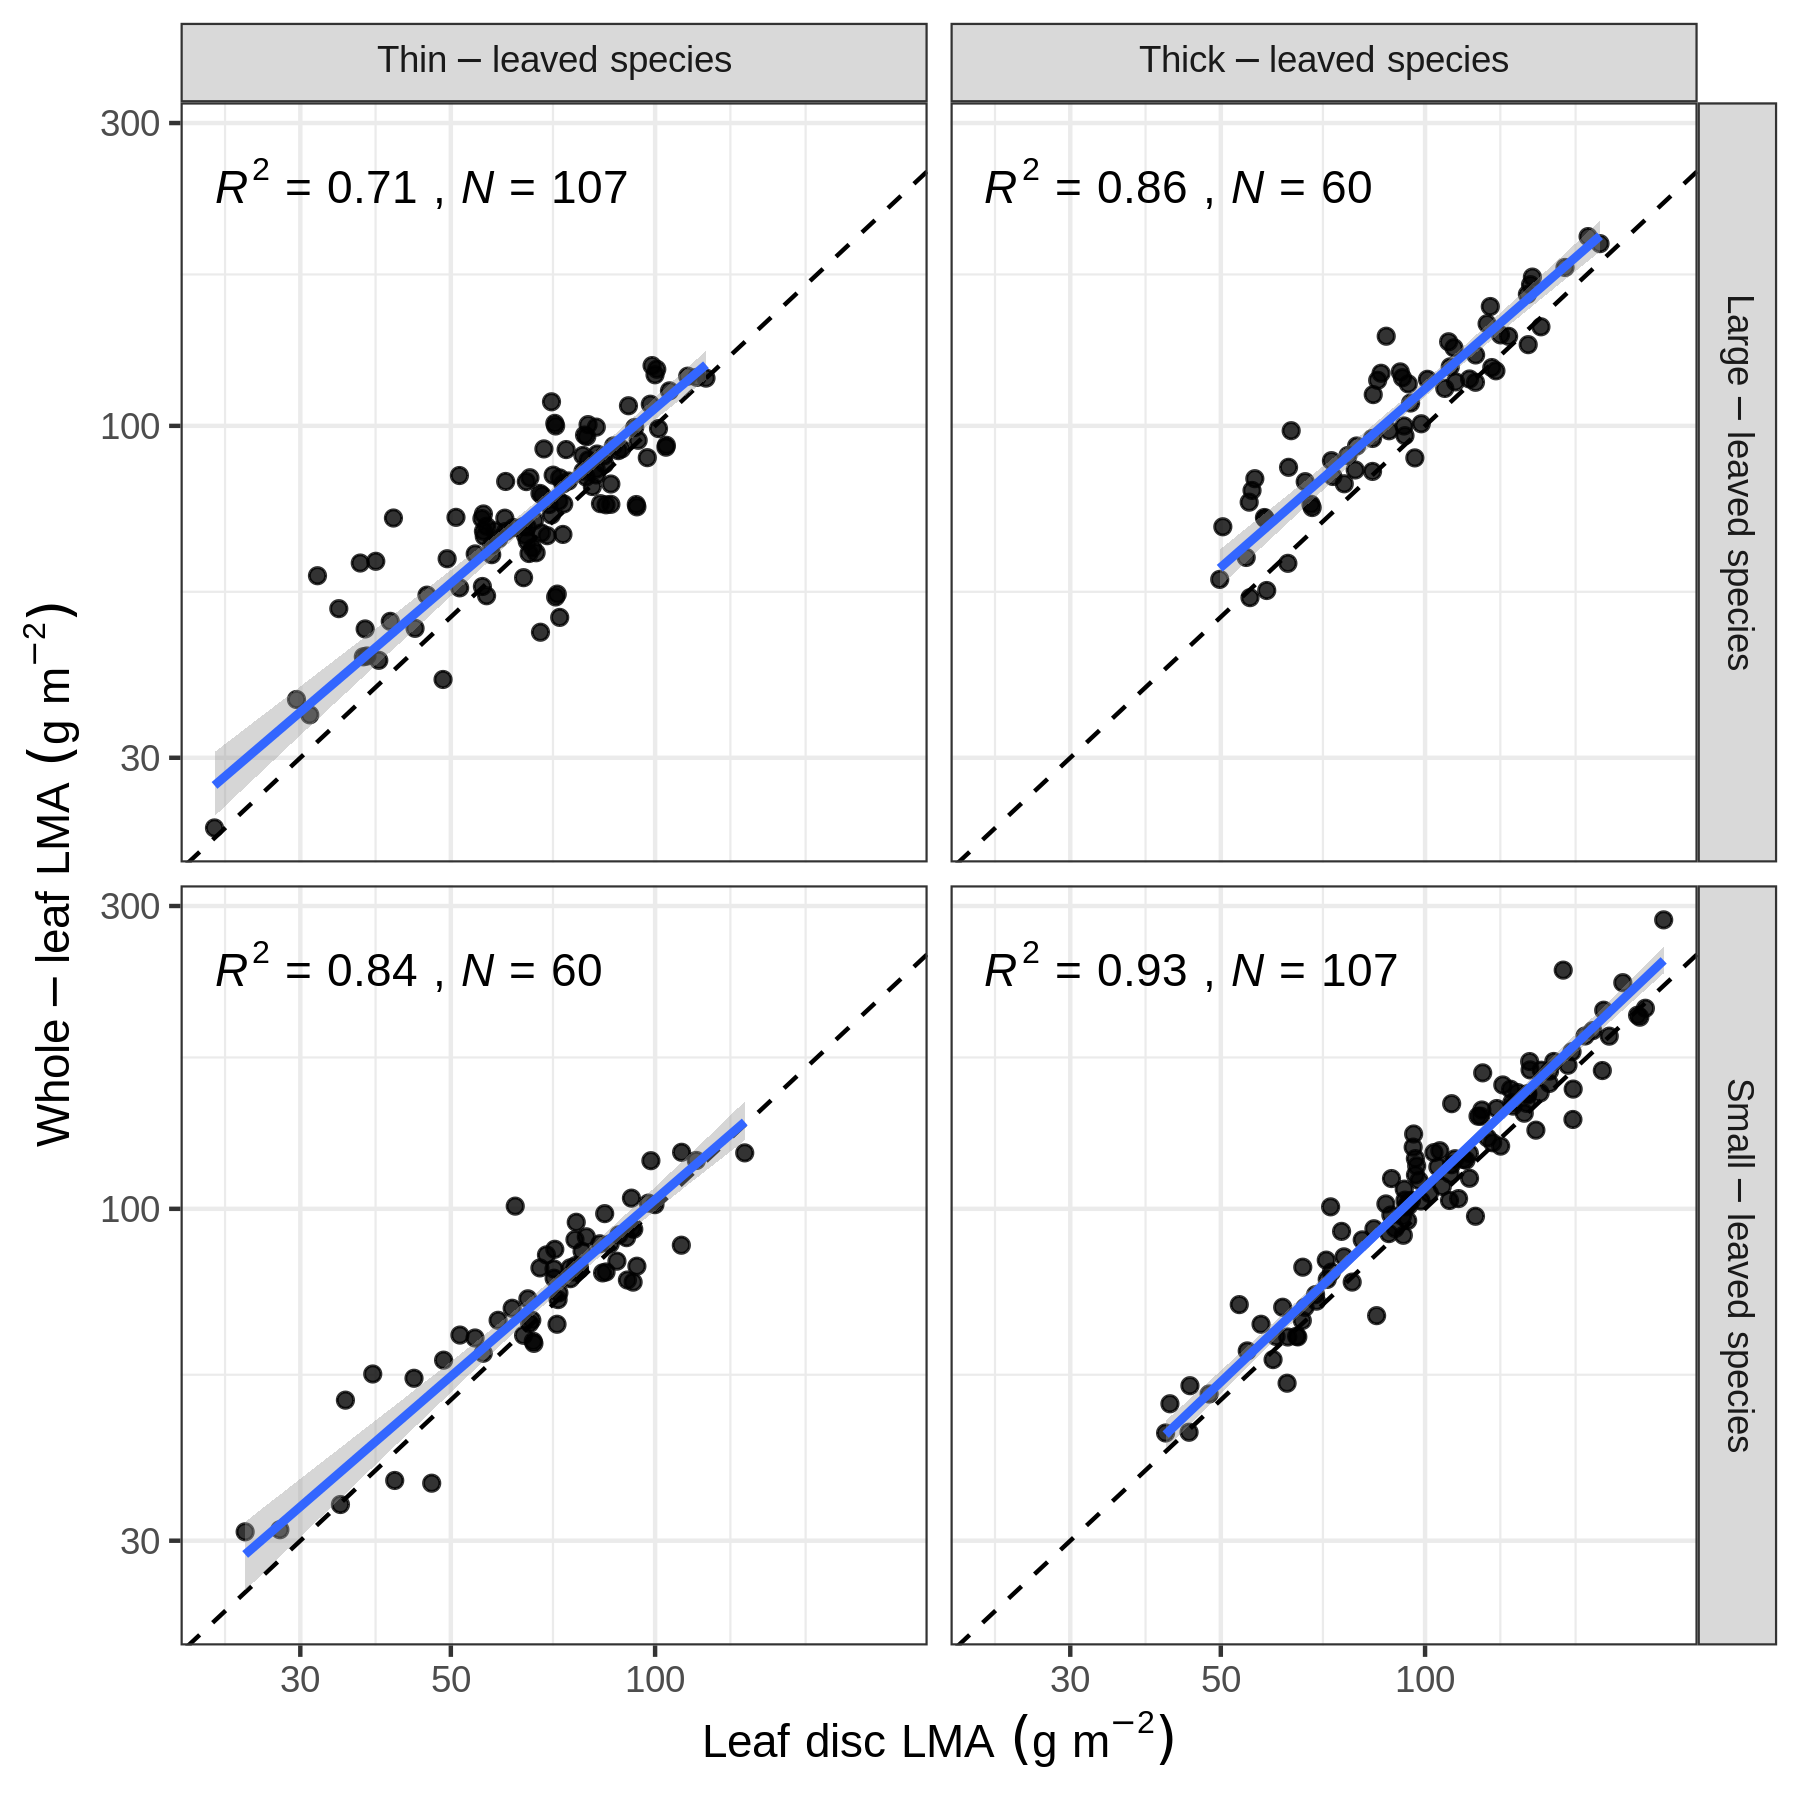
\includegraphics{../figs/lalt_pool_grid.png}

\newpage

\textbf{Fig. 2.} Relationships between individual leaf mass per area
(LMA) determined by using whole leaves and leaf discs. Individual groups
are divided into four categories based on the basis of the medians of
the leaf size and leaf thickness across all the individuals. All the
correlations are significant (\emph{P} \textless{} 0.001). Details as in
Fig. 1.

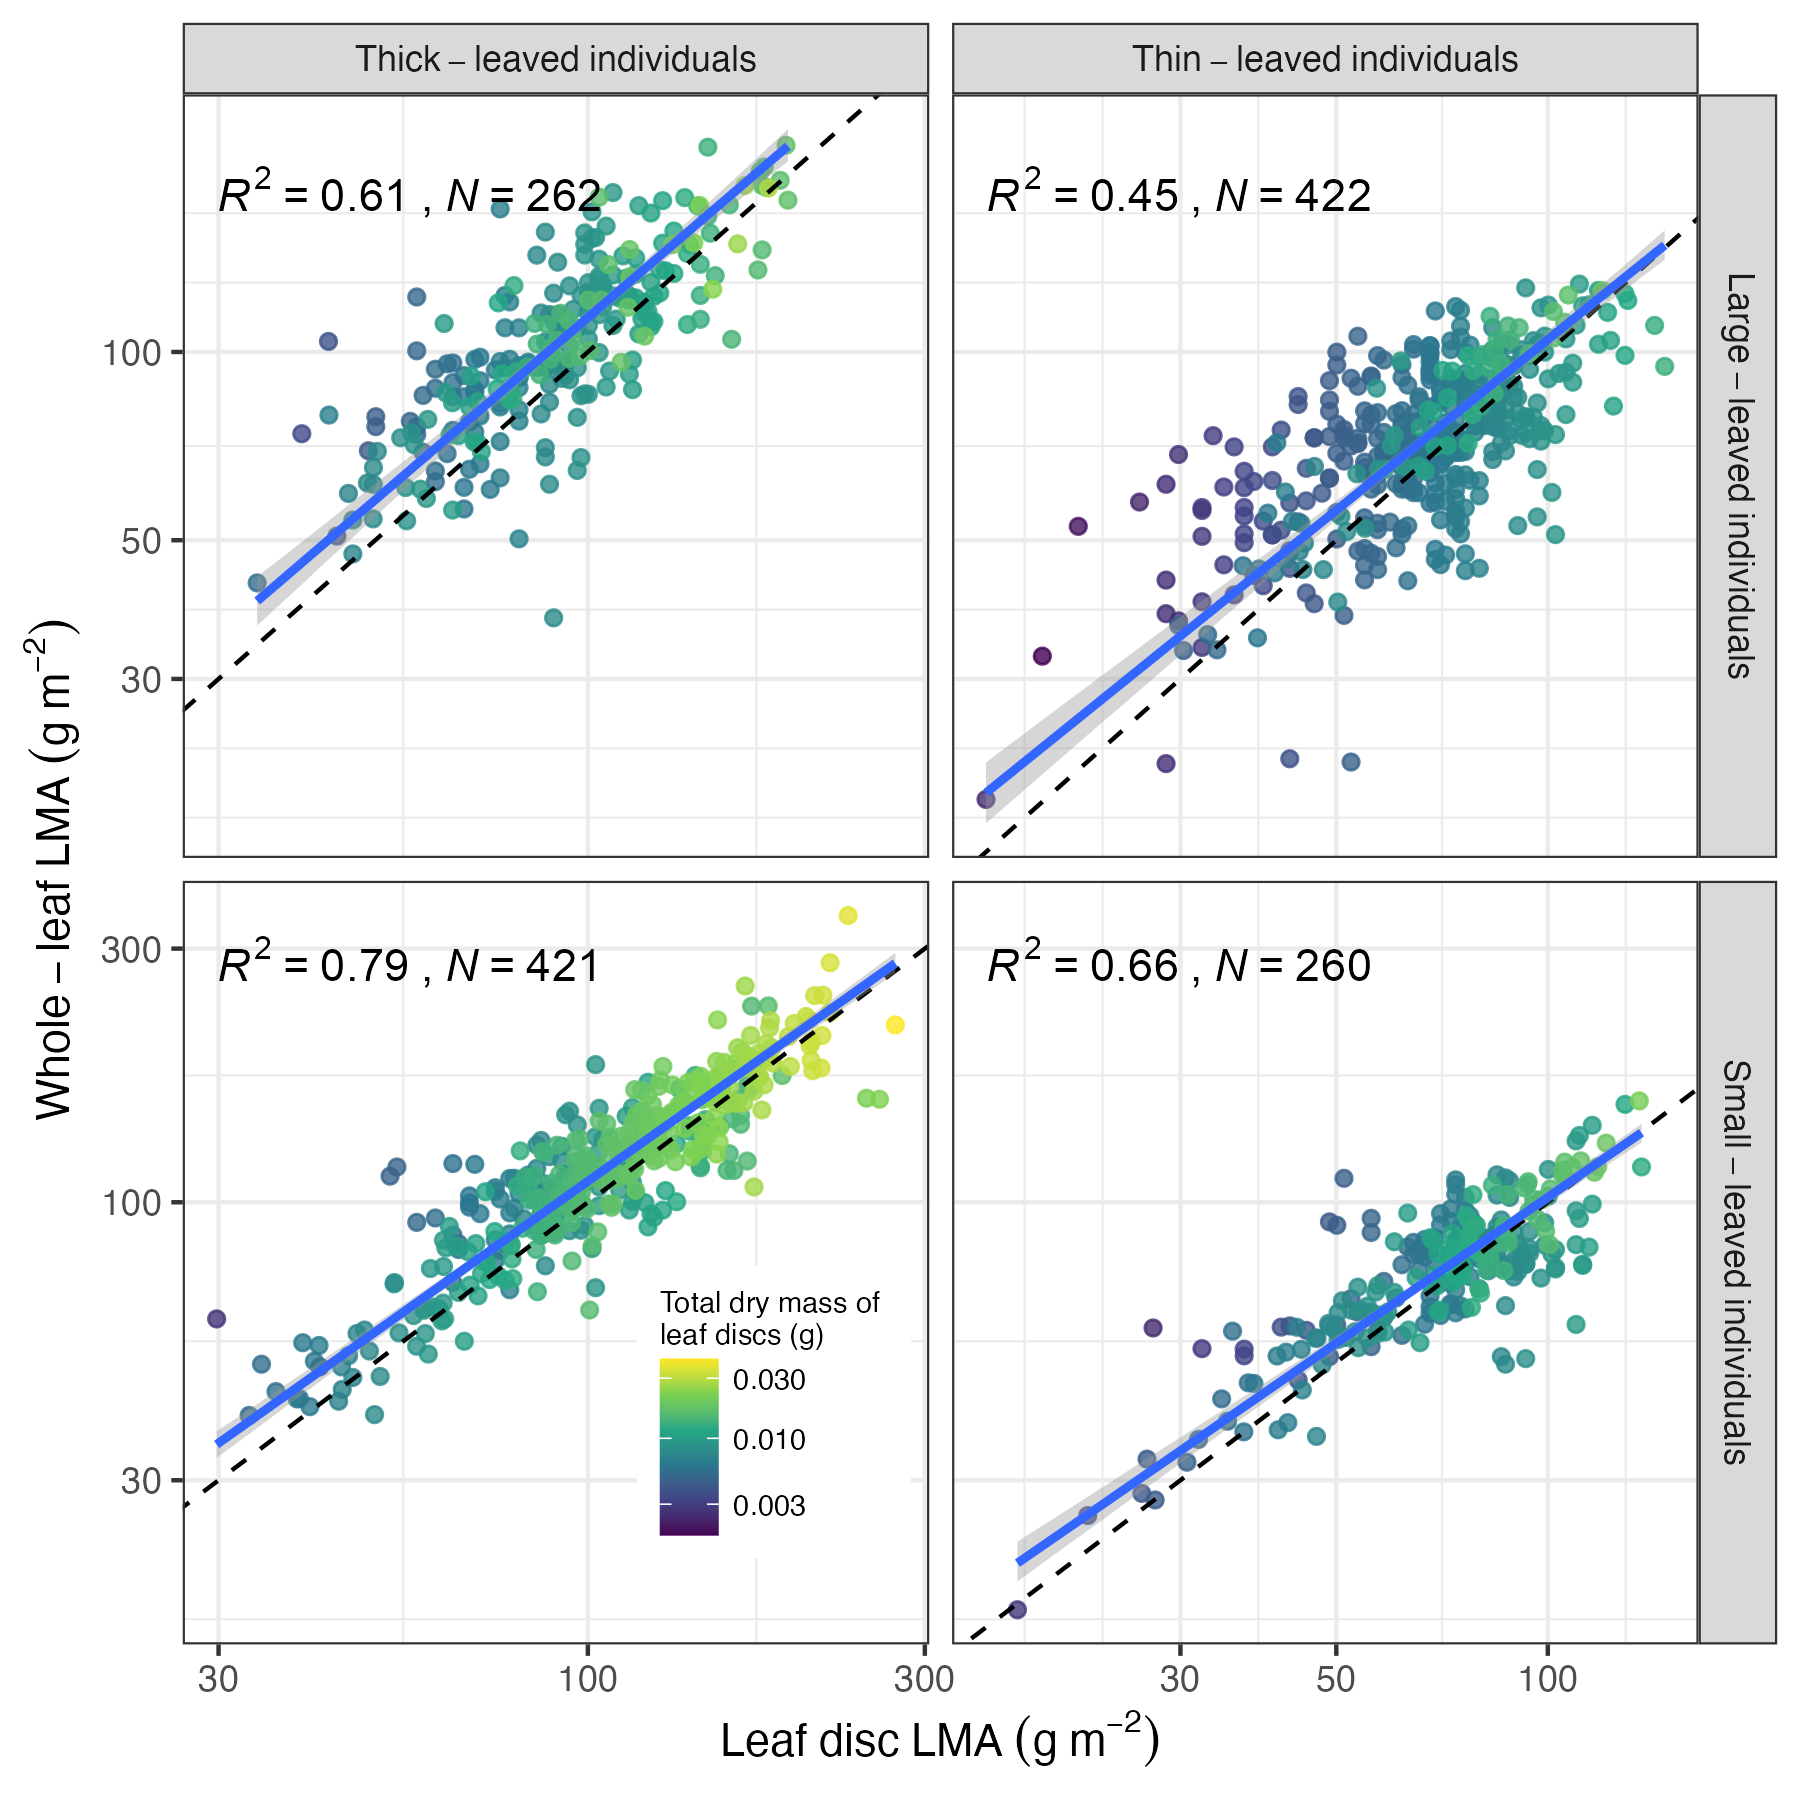
\includegraphics{../figs/lalt_tree_grid.png}

\newpage

\textbf{Fig. 3.} Relationships between coefficient of variation (CV) in
leaf trait values determined by using whole leaves and leaf discs: (a)
leaf mass per area (LMA). The correlation is significant (\emph{P}
\textless{} 0.001). Details as in Fig. 1. Note that the axes are square
root scales.

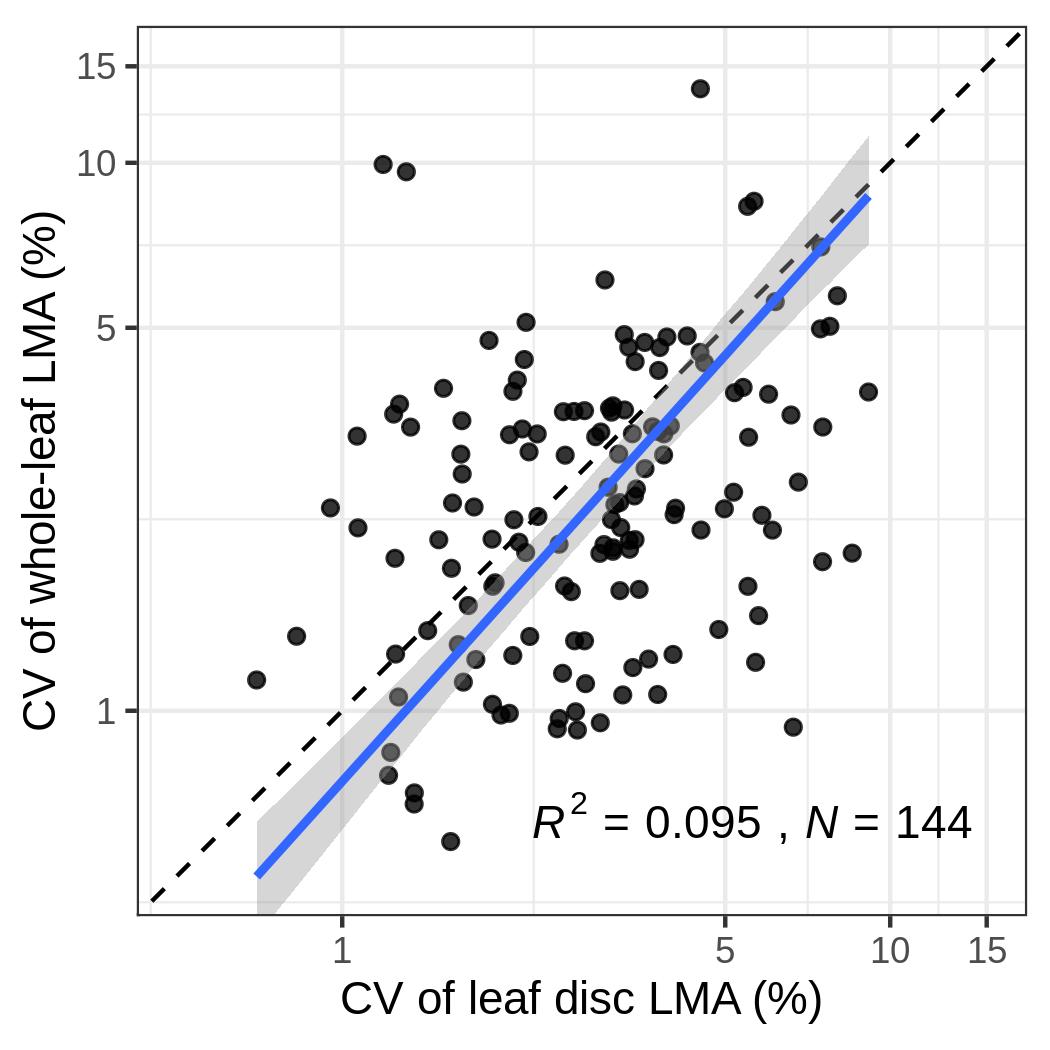
\includegraphics{../figs/cv_pool.png}

\end{document}
